\newpage

\section{Math 1166: Final Exam Review, Spring 2022 (draft)}

Note:  The final exam is cumulative, so be sure to include the \textbf{previous midterm review documents} as part of your review.  
Since the third midterm, we will have covered Sections 6.1 and 6.2 from your notes as well as Activities A.41 -- A.48, except A.44 and A.47.  (Some of these activities were modified for Desmos or GeoGebra.) Below is a summary of that content.  

Some of the following problems (as well as a few others) will be part of an online supplementary review, available by Reading Day.  

% A.40.Reading Information from a Graph
% A.41. Parametric Equations
% A.38.  Constructible Numbers (section 5.4) 
% Trig Checkup.  Circular trigonometry
% A.42. Parametric Plots of Circles
% A.44. Taxicab Distance (section 6.1)
% A.43. Eclipse the Ellipse
% A.45. City Geometry and Absolute Value
% A.47. Midsets Abound (section 6.2)
% A.48. Tenacity Paracity

%\subsection*{Coordinate Geometry}
%\begin{itemize}\itemsep-3pt
%\item What are the benefits of the standard form, the point-slope form, and the slope-intercept form of a line?  
%\item Find an equation of a line through a given point parallel to a given line.  (Try this in standard form.)  
%\item Find an equation of a line through a given point perpendicular to a given line.  (Try this in standard form.) 
%\item Given two lines, two circles, or a line and a circle, find their intersection(s) if any.  Describe what is happening geometrically when the algebra yields no solutions, exactly one solution, exactly two solution(s) or infinitely many solutions. 
%\item Given an equation of a circle or a parabola, complete the square to find the center of the circle or the vertex of the parabola.  
%%\item What are constructible numbers?  What are some numbers that are not constructible? 
%\end{itemize}

\subsection*{City Geometry}
\begin{itemize}\itemsep-3pt
\item Know the distance formula in city geometry, be able to use it, and explain its meaning. 
\item Given a center and a radius, graph a city-geometry circle and write its equation.  
\item Given two points in city geometry,  graph their midset and write an equation of the midset.  
\item Given a focus and a directrix, graph the city-geometry parabola and write its equation.  
\item Explain the absolute value function in several ways.
\item Graph and analyze absolute value equations (such as equations of city-geometry circles, midsets, or parabolas) by checking cases.  
\end{itemize}

\subsection*{Functions}
\begin{itemize}\itemsep-3pt
\item What is a function?  What do domain and range mean?  
\item Why is ``Is this a function?'' a poor question.  What is a better question?  
\item Graph and analyze parametric equations describing a path in the plane
\item In what sense are transformations of the plane functions?  What are the input and output values?  What are the domain and range of an isometry or dilation of the plane?  
\item Describe and analyze functions involving several related variables, such as length, width, area, and perimeter of rectangles.   When fixing one of these quantities, what kinds of functions can you find among the other quantities? 
\end{itemize}



%\subsection{Parametric Equations}
\subsection{Supplemental Review Problems}
Most of the problems below target content since the third midterm exam. 


\begin{prob}
Write an equation of the line through $(2,4)$ parallel to $5x-3y=1$.  
Now write an equation of the line through $(x_1,y_1)$ parallel to $ax+by=c$. 
\end{prob}

\begin{prob}
Write an equation of the line through $(2,4)$ perpendicular to $5x-3y=1$.  
Now write an equation of the line through $(x_1,y_1)$ perpendicular to $ax+by=c$. 
\end{prob}

\begin{prob}
Intersections of lines.  
\begin{enumerate}
%\item Find the intersection of the lines $2x-3y=4$ and $3x-5y=3$.  
%\item Find the intersection of the lines $2x-3y=4$ and $-4x+6y=-8$.
%\item Find the intersection of the lines $2x-3y=4$ and $-4x+6y=5$.
\item Find the intersection of the lines $2x-3y=5$ and $x+4y=19$.  
\item Find the intersection of the lines $2x-3y=5$ and $-4x+6y=7$.
\item Find the intersection of the lines $2x-3y=5$ and $-4x+6y=-10$.
\item How might you have predicted in advance how many solutions to expect for each previous system of equations?
\item Use algebra to help explain why lines intersect in zero, one, or infinitely many points.  (You know this geometrically, of course.  Here you demonstrate how algebra gives the same result.)  Indicate clearly the algebraic conditions
for which you get zero, one, or infinitely many points.  
\end{enumerate}
\end{prob}

\begin{prob}
Suppose you have a rectangle with vertices at $(0,0)$, $(a,0)$,
$(a,b)$ and $(0,b)$. Use algebra to prove that the diagonals have the
same length.
\end{prob}



%\begin{prob} 
%Consider a nonzero vector defined by the ordered pair $(a,b)$. Let $m$ be the magnitude (length) of this vector, \textbf{use algebra} to explain why
%\[
%\frac{(a,b)}{m}
%\]
%is a new vector whose magnitude is $1$ and whose direction is the same
%as $(a,b)$.
%\end{prob} 

%\begin{prob}
%Suppose you have a parametric plot defined by $x(t)$ and $y(t)$.
%\begin{enumerate}
%\item Compare and contrast the plots of
%\[
%\bigg(x(t),y(t)\bigg)\qquad\text{and}\qquad\bigg(x(t-6),y(t-6)\bigg).
%\]
%\item Suppose that there are two bugs whose positions are given by:
%\[
%\mathrm{bug}_1(t) = \bigg(x(t),y(t)\bigg)\qquad\text{and}\qquad\mathrm{bug}_2=\bigg(x(t-6),y(t-6)\bigg).
%\]
%where $t$ represents time in seconds. Describe what happens as $t$
%runs from $0$ seconds to $36$ seconds.
%
%\item Now suppose that there are two bugs whose positions are given
%  by:
%\[
%\mathrm{bug}_1(t) = \bigg(x(t),y(t)\bigg)\qquad\text{and}\qquad\mathrm{bug}_2=\bigg(x(t)-6,y(t)-6\bigg).
%\]
%where $t$ represents time in seconds. Describe what happens as $t$
%runs from $0$ seconds to $36$ seconds.
%\end{enumerate}
%\end{prob} 

\begin{prob}
Find the intersection of the lines
\begin{align*}
x_1(t) &= -6 + 9t & x_2(t) &= 3+t \\
y_1(t) &= 3-2t &  y_2(t) &= -4-2t 
\end{align*}
If $(x_1(t),y_1(t))$ gives the position of $\mathrm{jogger}_1$ and
$(x_2(t),y_2(t))$ gives the position of $\mathrm{jogger}_2$, what is
the significance of the point of intersection of these lines, from the
perspective of the joggers?
\end{prob}

\begin{prob}
A bug moves according to the following parametric equations, where t is measured in seconds and $x$ and $y$ are measured in centimeters:  $x = 2t^2$, $y = t-2$.  (Suppose $t$ can be any real number.)   
\begin{enumerate}
\item Describe the path of the bug.  
\item Is the bug's position a function of time?  
\item On the path, is $y$ a function of $x$?  
\item Is $x$ a function of $y$?  
\item If you know one of $x$, $y$, or $t$, can you determine the other two?  How does this question relate to the previous two questions?  
\item In school mathematics, students are often given a graph and asked, ``Is it a function.''  Explain why this is a poor question.  What better questions could you ask?  
\end{enumerate}
\end{prob}

%\subsection{Absolute Value, Distance, and City Geometry}
\begin{prob}
Consider the following equations:  
\setlength{\arraycolsep}{12pt}
\setlength{\extrarowheight}{3pt}
\[
\begin{array}{cccc}
x^2-y^2=0    &   x^2=y^2   &   |y|=|x|   &   y= \pm x \\
(x-y)(x+y)=0  &   x= \pm y   &   y = \pm|x|   & x = \pm|y|
\end{array}
\]
\begin{enumerate}
\item Which equations are equivalent to which other equations?  Say how you know.  (Be sure to state what it means for the equations to be equivalent.)
\item For each set of equivalent equations, graph the solution set, and describe how each of the equations provides a different way about thinking about that solution set.  
\end{enumerate}
\end{prob}

\begin{prob}
Distance formulas and circle equations across dimensions.  
\begin{enumerate}
\item What is the (Euclidean) distance formula in 2 dimensions, on the $xy$-plane?  
\item What is the distance formula in 3 dimensions?
\item What is the distance formula in 1 dimension?
\item Write an equation of the circle of radius $r$ and center $(a, b)$.  
\item Explain how a circle is a one-dimensional figure living in a two-dimensional ``space.''
\item In three-dimensional space, write an equation of the two-dimensional ``circle'' of radius $r$ and center $(a, b, c)$.  
\item In one-dimensional space, write an equation of the zero-dimensional ``circle'' of radius $r$ and center $a$.  
\end{enumerate}
\end{prob}

%\begin{prob}
%Distances across dimensions.  
%\begin{enumerate}
%\item Find all numbers that are equidistant from 3 and 8.  
%\item Find all points $(x, y)$ that are equidistant from $(3, 0)$ and $(8, 0)$.  
%\item Find all points $(x, y, z)$ that are equidistant from $(3, 0, 0)$ and $(8, 0, 0)$.  
%\item Find all real numbers that are twice as far from 3 as they are from 8.
%\item Find all points $(x, y)$ that are twice as far from $(3, 0)$ as they are from $(8, 0)$.
%\item Find all points $(x, y, z)$ that are twice as far from $(3, 0, 0)$ as from $(8, 0, 0)$.
%\end{enumerate}
%\end{prob}
%
%4.5.  One way of solving problems 4a and 4d is as follows: 
%(1)	Use a distance formula from problem 3 to express the distances from x to 3 and from x to 8; 
%(2)	Use an equation to relate the distances from part (1); and 
%(3)	Thinking of the two sides of the equation as functions, graph the two functions and look for intersections of the graphs. 
%How can you use this approach to predict how many solutions you will find?

\begin{prob} 
Recall the method in Euclidean geometry of constructing an equilateral triangle on a given segment.  Suppose a ``city geometry compass'' draws a city geometry circle.  Imagine using such a ``city geometry compass'' below.  
\begin{enumerate}
\item Construct a ``city geometry equilateral triangle'' on the segment defined by the
  points $(0,0)$ and $(4,0)$. Explain your steps.
\item Now construct a ``city geometry equilateral triangle'' on the segment defined by the
  points $(0,0)$ and $(2,2)$. Explain your steps.
\item Will the construction always give a (unique!) equilateral triangle? What does ``unique'' mean in this context? Give a detailed discussion.  
\end{enumerate}
\end{prob} 


\fixnote{Add problems about oriented area, planimeter.}  

%
%\begin{prob}
%Using oriented area, given a quadrilateral $ABCD$, and any point $O$ in the plane, $$\text{area} ABCD = \text{area}\triangle OAB + \text{area}\triangle OBC + \text{area}\triangle OCD + \text{area}\triangle ODA.$$
%\end{prob}
%  
%\begin{prob}
%A parallelogram with vertices at $(0,0)$, $(a,b)$, $(c,d)$, and $(a+c,b+d)$ has (oriented) area $ad-bc$. 
%% Draw a big rectangle around it, and subtract the stuff we don't want.
%% Row reduction of a matrix as parallelograms with same base, same height.  Area (and determinant) is constant.  
%\end{prob}
%
%\begin{prob}
%If $ad-bc = 0$, then $(a,b)$ and $(c,d)$ are parallel.  What about the converse?  
%\end{prob}

\begin{prob}
A fundamental feature of the basic rigid motions in Euclidean geometry is that they preserve distance and angle.  In city geometry, some basic rigid motions preserve both distance and angle and others fail for various reasons.  Explain.  (Hint:  Some but not all rotations preserve both distance and angle.)  
\end{prob}

%\begin{prob} 
%Clearly identify which of the following numbers are constructible and
%which numbers are not constructible.
%\[
%4 \qquad  \sqrt[3]{2} \qquad3.1415926 \qquad \sqrt[3]{125} \qquad \sqrt[6]{7} \qquad \frac{6}{1+\sqrt{5}}
%\]
%\end{prob}

\begin{prob}
Consider $x=(y-2)^2+3$. 
\begin{enumerate}
\item Plot this curve.  
%\[
%\includegraphics{complexPlane.pdf}
%\]
\item Explain how this might not be the plot of a function.

\item Explain how this could be the plot of a function.
\end{enumerate}
\end{prob}


\begin{prob} 
Below are two points in City Geometry. 
\[
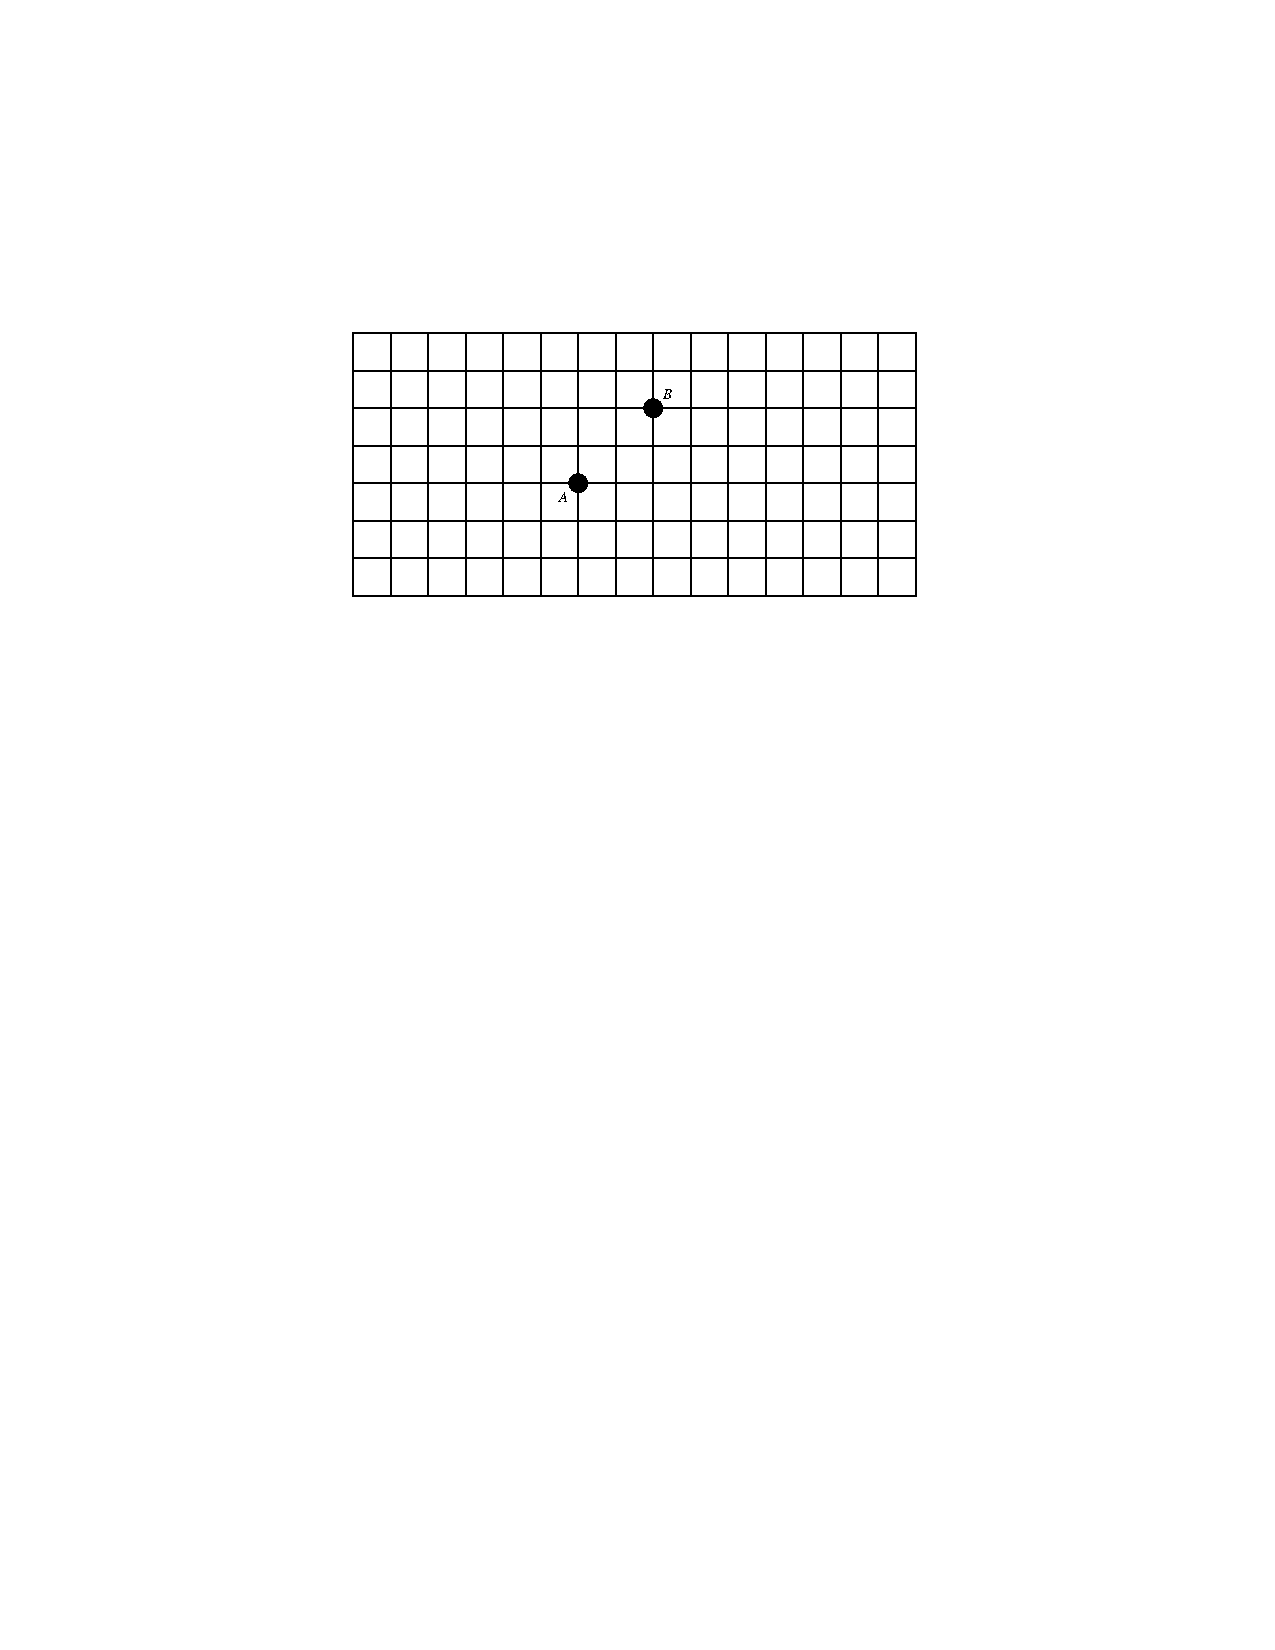
\includegraphics{1166finalmidset.pdf}
\]
\begin{enumerate}
\item Sketch the City Geometry midset of these two points.  
\item Suppose that $A=(0,0)$ and $B=(2,2)$.  Using taxicab distance in City Geometry, write an equation that must be satisfied by any point $(x,y)$ that is in the midset of $A$ and $B$.  
\item Explain the connection between the geometry in part (a) and the algebra in part (b) for the case $x > 2$ and $y < 0$.  
\end{enumerate}
\end{prob}

\begin{prob}
Use coordinate constructions to derive the formula for the parabola
whose focus is the point $(-3,-4)$ and whose directrix is the line $y
= 2$. Show your work. Note, you should use the Euclidean distance
formula, and your final answer should start with ``$y = $''.  
\end{prob}

\begin{prob}
Comparing Celsius and Fahrenheit.  
\begin{enumerate}
\item Water freezes at $0^\circ$ C, which is $32^\circ$ F.  Water boils at $100^\circ$ C, which is $212^\circ$ F.  Use this information to derive a Celsius to Fahrenheit conversion formula.  
\item Suppose the temperature of a model house increases from $24^\circ$ C to $30^\circ$ C, which seems to be a $25\%$ increase.  Convert these temperatures to Fahrenheit and compute the percent change in degrees Fahrenheit. 
\item Use your conversion formula to explain why the percent changes are not the same in Fahrenheit as in Celsius.  
\end{enumerate}
\end{prob}


\begin{prob}
Surface area of a cylinder.
\begin{enumerate}
\item Derive and explain a formula for the surface area of a right cylinder of radius of radius $r$ and height $h$.  
\item Assuming the radius is fixed, how does the surface area vary with the height?  In other words, what kind of function is it?  Explain briefly.  
\item Assuming the height is fixed, how does the surface area vary with the radius?  Explain briefly. 
\end{enumerate}
\end{prob}

\begin{prob}
Volume of a cylinder.
\begin{enumerate}
\item Derive and explain a formula for the volume of a right cylinder of radius of radius $r$ and height $h$.  
\item Assuming the radius is fixed, how does the volume vary with the height?  In other words, what kind of function is it?  Explain briefly.  
\item Assuming the height is fixed, how does the volume vary with the radius?  Explain briefly. 
\end{enumerate}
\end{prob}


%\begin{prob}
%Standard televisions usually have an aspect ratio (width:length) of 4:3.  Wide-screen televisions have an aspect ratio of 16:9.  Brad's first wide-screen television was a 36 inch (diagonal) model.  Although the new television was clearly wider than the 27 inch (diagonal) standard television it replaced, he was surprised that it did not seem taller than the old television.  Which television was actually taller or shorter?  By how much?  Explain your reasoning.   
%\end{prob}

%\begin{prob}
%Given an equation of a line in standard form, $ax+by=c$:  
%\begin{enumerate}
%\item Find an efficient way to write down an equation of a perpendicular line through the point $(p,q)$.  
%\item Explain why efficient the method works. 
%\end{enumerate}
%\end{prob}

\begin{prob}
Below is a figure that illustrates part of Euclid's proof of the Pythagorean Theorem.  You may assume the following: 
\begin{itemize}
\item All  angles that appear to be right angles are indeed right.
\item $FB=BA$ and $BD=BC$. 
\item $\triangle ABD \cong \triangle FBC$.  
\end{itemize}
\[
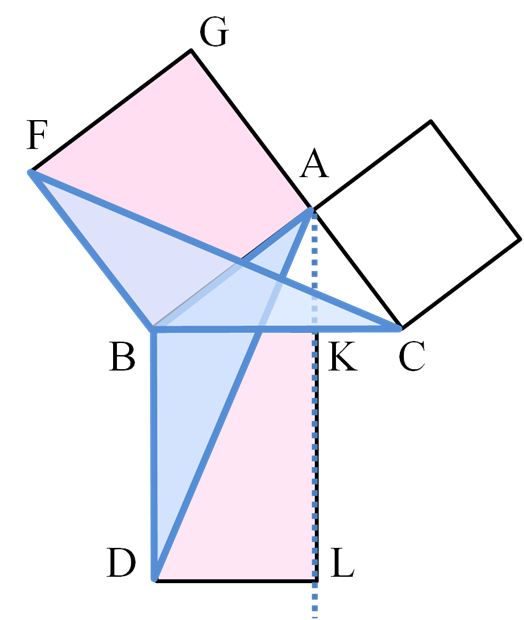
\includegraphics[scale=0.25]{../graphics/Euclid_Pythagorean_theorem3.PNG}
\]
\begin{enumerate}
\item Why is the area of $\triangle KBD$ (not drawn) equal to the area of $\triangle ABD$?
\item Why is the area of $\triangle FBC$ equal to the area of $\triangle FBA$ (not drawn)?
\item Explain briefly why the area of rectangle $KBDL$ equal to the area of rectangle $FBAG$.
\item Now explain how to complete the proof of the Pythagorean theorem.  \end{enumerate}
\end{prob}


%\begin{prob}
%Using the picture below, prove that if two non-vertical lines are perpendicular, the product of their slopes is $-1$.   You may assume that $x$ and $y$ are horizontal and vertical axes, respectively; that lines $j$ and $k$ are perpendicular and that $j$ has positive slope; that the segments of length $a$ and $c$ are vertical and collinear; and that the segment of length $b$ is horizontal.   
%$$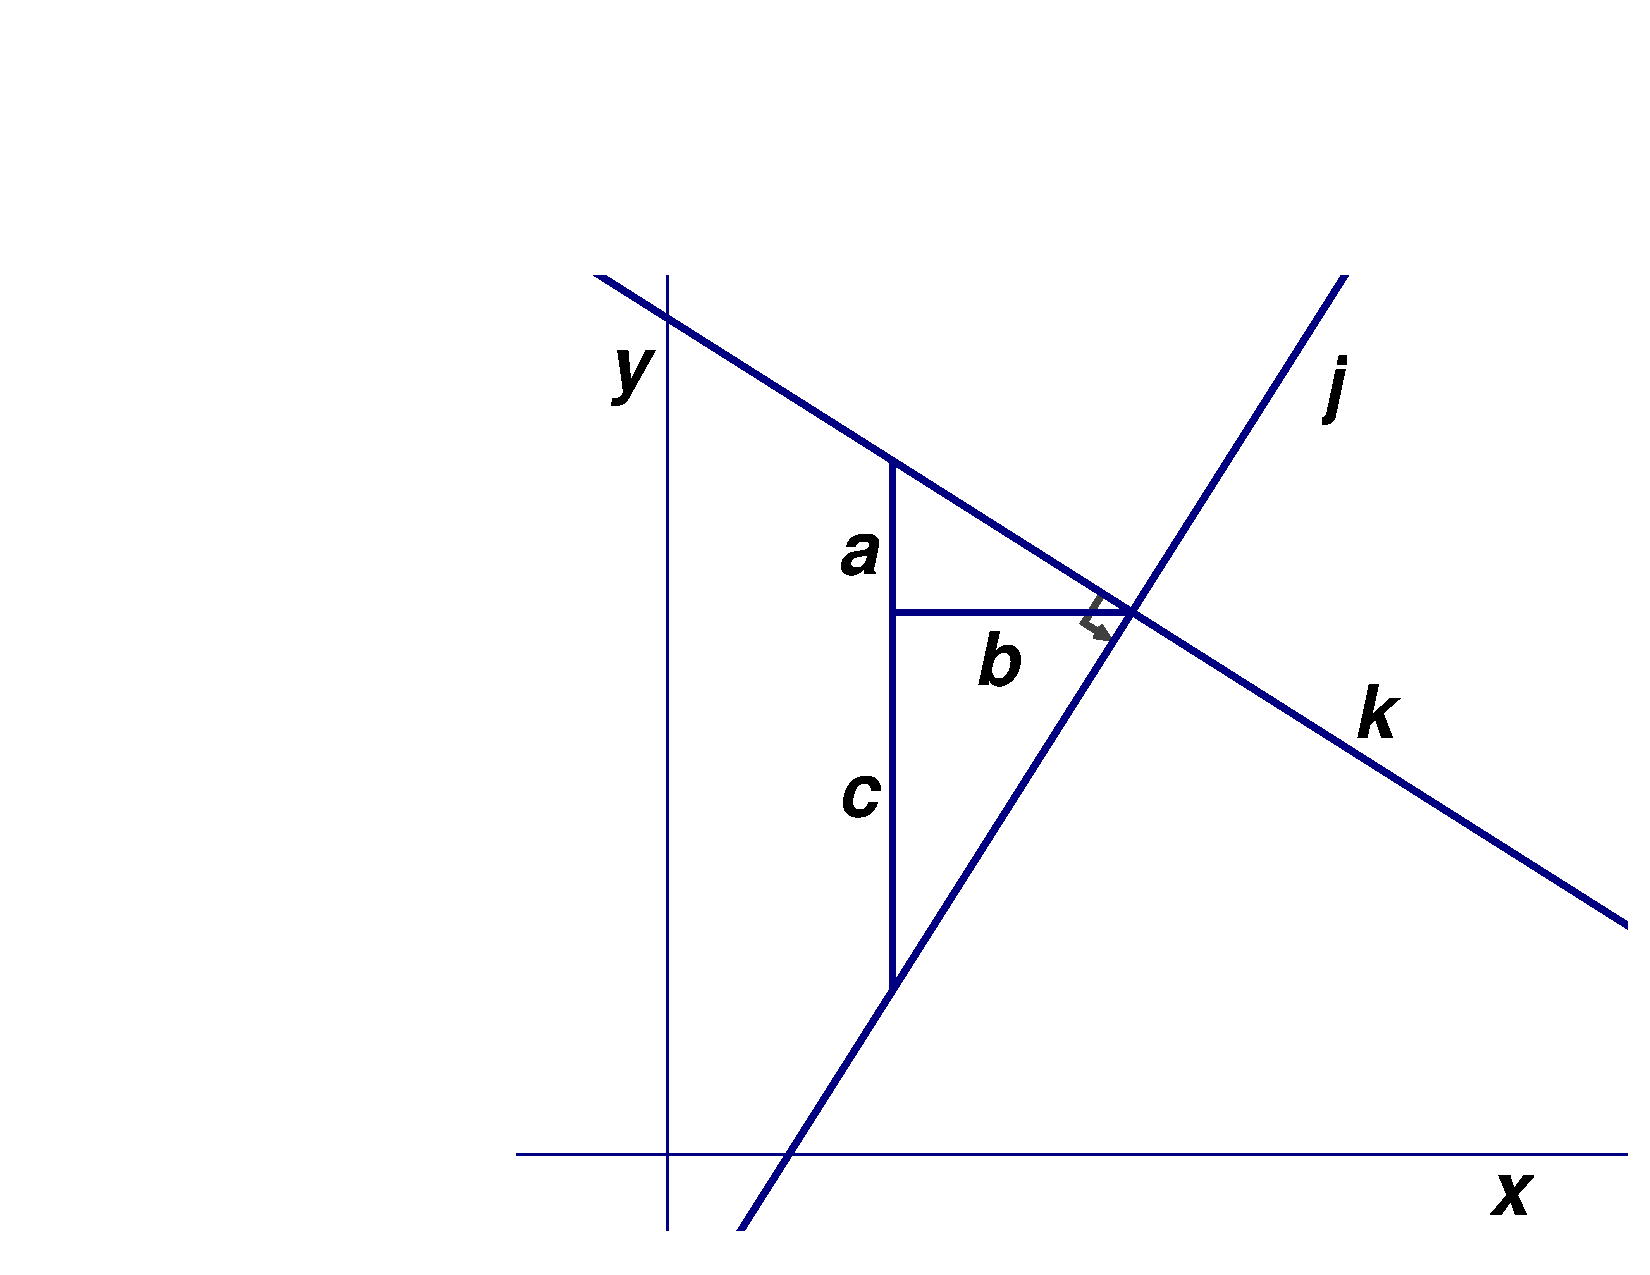
\includegraphics[width=2.5in]{../graphics/perpendicularSlopes.pdf}$$
%\end{prob}

%\subsection*{Questions to be added}
%\begin{enumerate}
%\item Vertex of parabola, completing the square
%\item Trigonometry
%\item Reason with letters.
%\item Solve for different letters.
%\item Different units, measurement
%\item number of solutions 
%\end{enumerate}

